%& --translate-file latin2pl
\documentclass{article}

\usepackage{polski}
\usepackage{hyperref}
\usepackage[T1]{fontenc}
\usepackage[utf8]{inputenc}
\usepackage{listings}
\hypersetup{
colorlinks=true,
urlcolor=blue,
}
\setcounter{section}{-1}
\lstset{
basicstyle=\fontsize{6}{6}\selectfont\ttfamily,
}
\usepackage{graphicx}
\graphicspath{ {./images/} }
\usepackage[a4paper, total={6in, 8in}]{geometry}

\title{
Lekizapteki\\
\large architektura}
\author{Marcin Abramowicz \and Mateusz Danowski \and Dawid Jamka \and Tomasz Patyna}


\begin{document}
  \maketitle

  \section{Dziennik zmian}
    \begin{tabular}{|c|c|c|}
      Nr iteracji & Data & Opis zmian \\
      \hline
      1. & 25.03.2020 & Utworzenie dokumentu oraz jego pierwsza wersja. \\
      \hline
      1. & 29.04.2020 & Poprawki w endpointach i schema. \\
      \hline
      2. & 29.06.2020 & Współczynnik opłacalności w wyświetlanej tabeli oraz mała modyfikacja api. \\
    \end{tabular}

  \section{Ogólna struktura}
    Aplikacja składa się z frontendu WWW napisanego w
    \href{https://angular.io}{Angularze}, backendu napisanego w
    \href{https://spring.io}{Spring Framework} oraz bazy danych
    \href {https://www.h2database.com/html/main.html}{H2}.

  \section{Komunikacja}
    \subsection{Backend - Baza Danych}
    Backend komunikuje się z lokalną bazą danych dzięki
    \href{https://hibernate.org}{Hibernate} oraz
    \href{https://spring.io/projects/spring-data-jpa} {Spring Jpa}.
    Framework zajmuje się konstruowaniem zapytań oraz tworzeniem schematu bazy danych.

    \subsection{Frontend - Backend}
    Komunikacja jest synchroniczna i odbywa się protokołem HTTP, serwer dostarcza
    \href{https://en.wikipedia.org/wiki/Representational_state_transfer}{RESTful API},
    obsługując żądania w formacie
    \href{https://en.wikipedia.org/wiki/JSON}{json}.
    Serwer jest dostępny na ``Google cloud'' na porcie 7312
    natomiast frontend wykonuje zapytania za pomocą
    \href{https://angular.io/guide/http}{HttpClient'a} służącego do wykonywania zapytań http.
    Nie ma stosowanych żadnych form zabezpieczeń, żądania i odpowiedzi nie są szyfrowane, ani nie ma wymiany tokenów.
    API backendu jest publiczne, więc każdy dysponujący linkiem może z niego korzystać.
    Backend akceptuje jedynie zapytania w formacie \texttt{application/json}.
    Odpowiedzi również są jedynie w formacie \texttt{application/json}
    Oznacza to, że zapytania do backendu powinny być z nagłówkiem: \texttt{Accept: application/json},
    natomiast odpowiedzi będą z nagłówkiem: \texttt{Content-Type: application/json}.

    \subsubsection{Endpointy udostępniane przez backend}
    \noindent
    \begin{minipage}{.45\textwidth}
     \begin{lstlisting}
       - GET /lekizapteki/diseases

         Response:
         HTTP/1.1 200 (OK)
         Body:
         [{
           "id": Long,
           "name":"String"
         }]


       - GET /lekizapteki/medicines

         Parameters:
         diseaseId: Long (optional)

         Responses:
         HTTP/1.1 200 (OK)
         Body:
         [{
           "ean": "String",
           "name": "String",
           "dose": "String"
         }]

         HTTP/1.1 404 (Not Found)
         Message: "Nieprawidlowa jednostka chorobowa"

       - complex types definitions
         PricingDto: {
           "tradePrice": Decimal,
           "salePrice": Decimal,
           "retailPrice": Decimal,
           "totalFunding": Decimal,
           "chargeFactor": Decimal,
           "refund": Decimal,
           "isLumpSum": boolean,
           "isFree": boolean,
           "profitabilityRate": Decimal
        }

     \end{lstlisting}
    \end{minipage}\hfill
    \begin{minipage}{.45\textwidth}
      \begin{lstlisting}
          MedicineDto: {
            "ean": "String",
            "name": "String",
            "activeIngredient": String
            "dose": "String",
            "form": "String",
            "pricing": PricingDto
          }

        - GET /lekizapteki/medicines/identical

          Parameters:
          ean: String
          diseaseId: Long (optional)

          Responses:
          HTTP/1.1 200 (OK)
          Body:
          {
            "medicine": MedicineDto,
            "identicalMedicines: [MedicineDto]
          }

          HTTP/1.1 404 (Not Found)
          Message: "Nieprawidlowy numer EAN"

          HTTP/1.1 404 (Not Found)
          Message: "Lek o podanym numerze EAN nie jest
            przepisywany na wybrana jednostke chorobowa"
      \end{lstlisting}
    \end{minipage}

  \section{Frontend}
  Frontend jest dostępny na
  \href{http://students.mimuw.edu.pl:1237}{serwerze Students na porcie `1237`} i jest publiczny,
  każdy dysponujący linkiem może z niego korzystać.
  Użytkowanie nie wymaga zakładania konta ani autoryzacji.

  Frontend posiada web serwis oraz modele odpowiadające odbieranym danym z backendu.
  Do tworzenia elementów używane są wbudowane komponenty oraz odpowiednie komponenty ogólnodostępne w internecie.

    \subsection{Makiety}
      \subsubsection{Wybór choroby}
      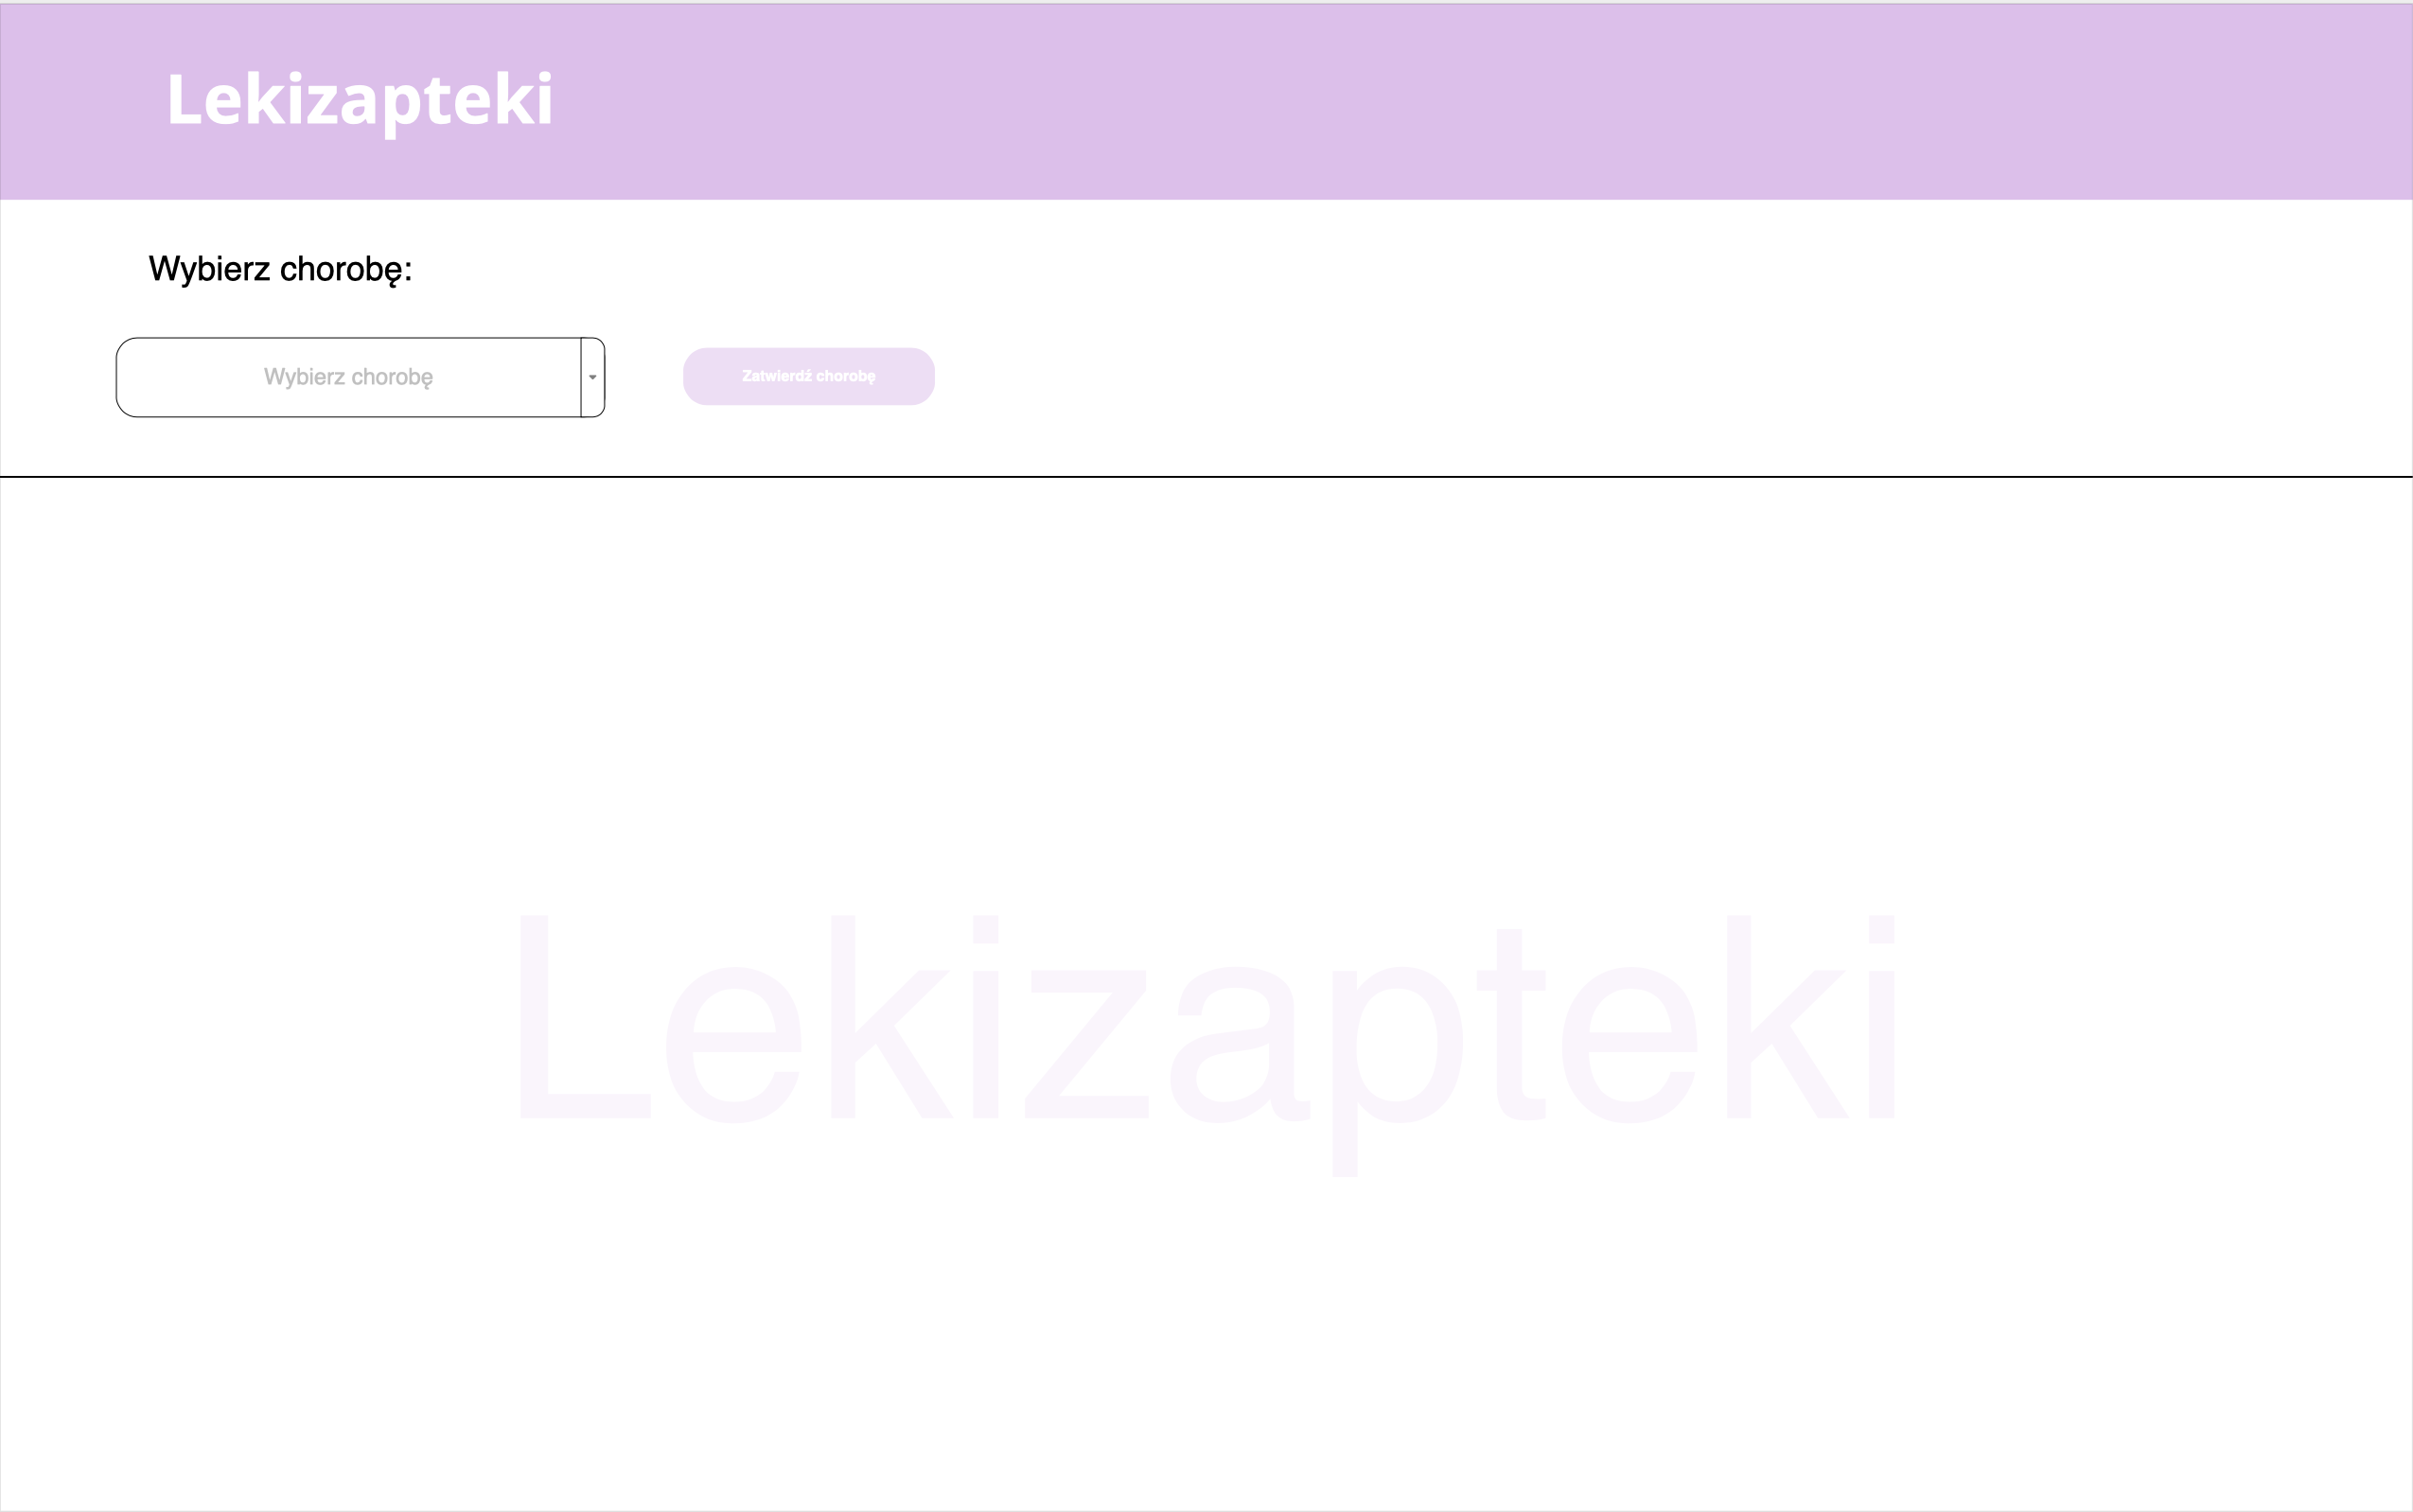
\includegraphics[width=8cm]{images/lekizapteki-wybor-choroby}

      \subsubsection{Wybór leku za pomocą nazwy i numeru EAN}
      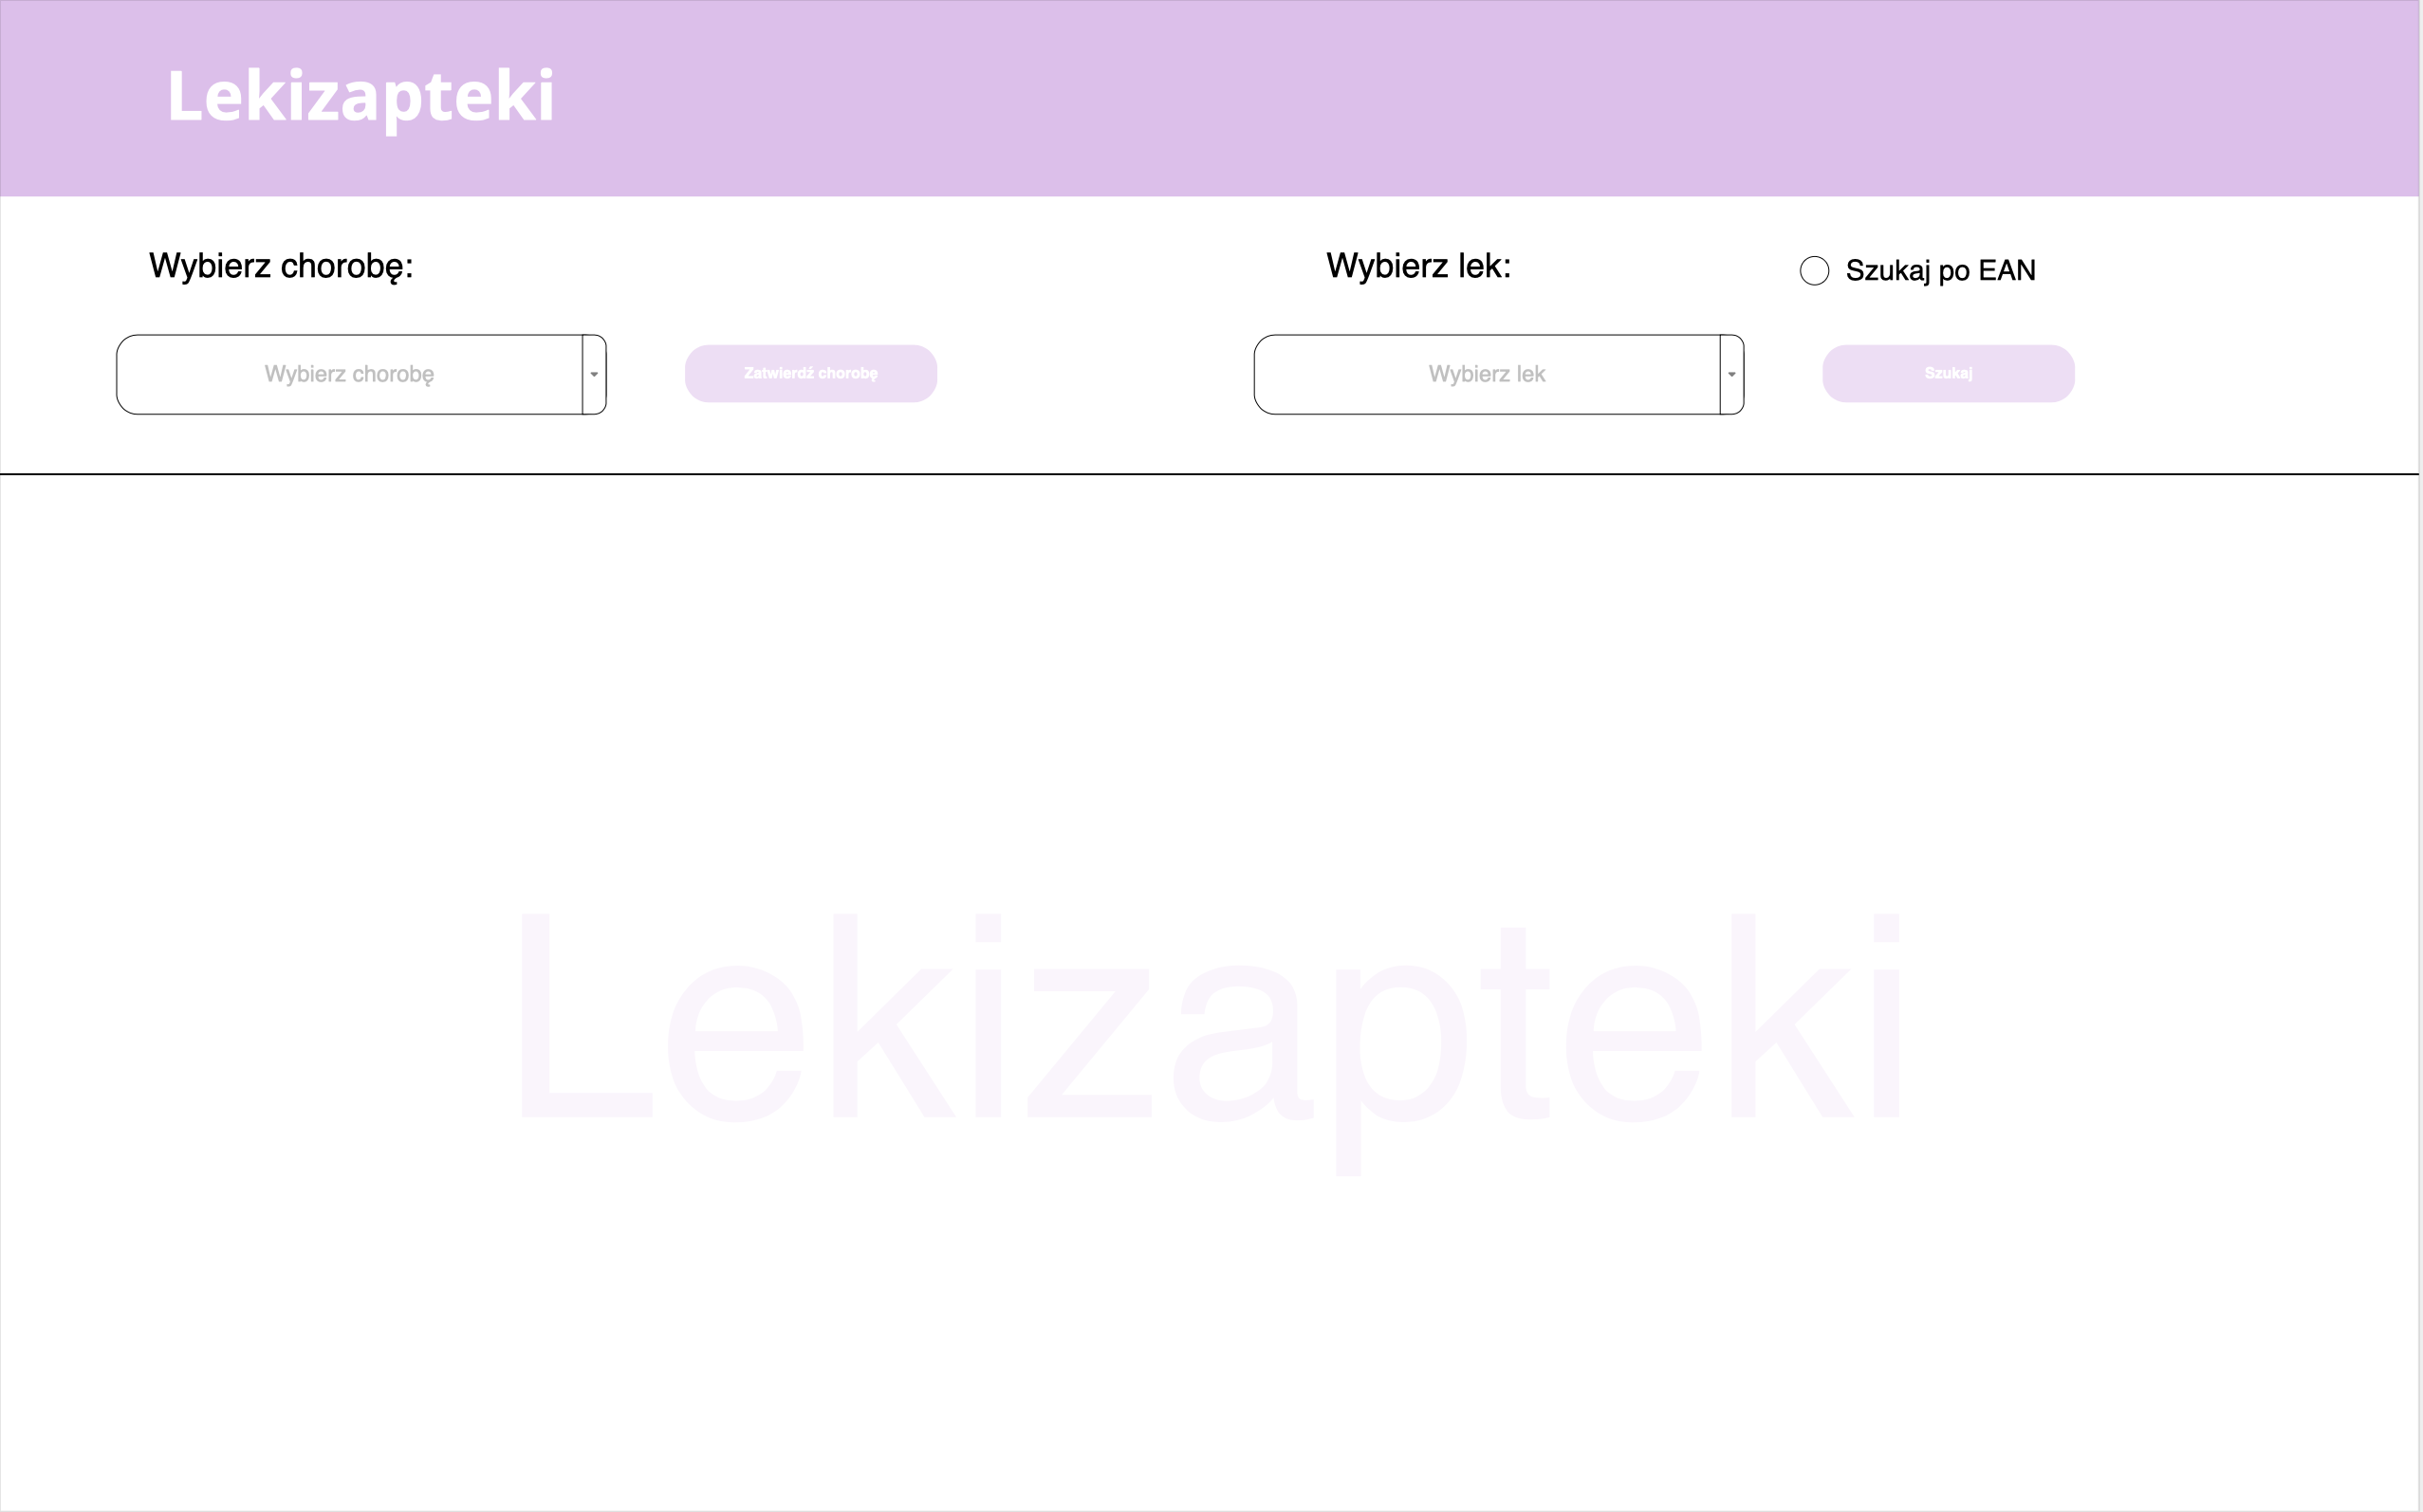
\includegraphics[width=8cm]{images/lekizapteki-wybor-leku-nazwa}
      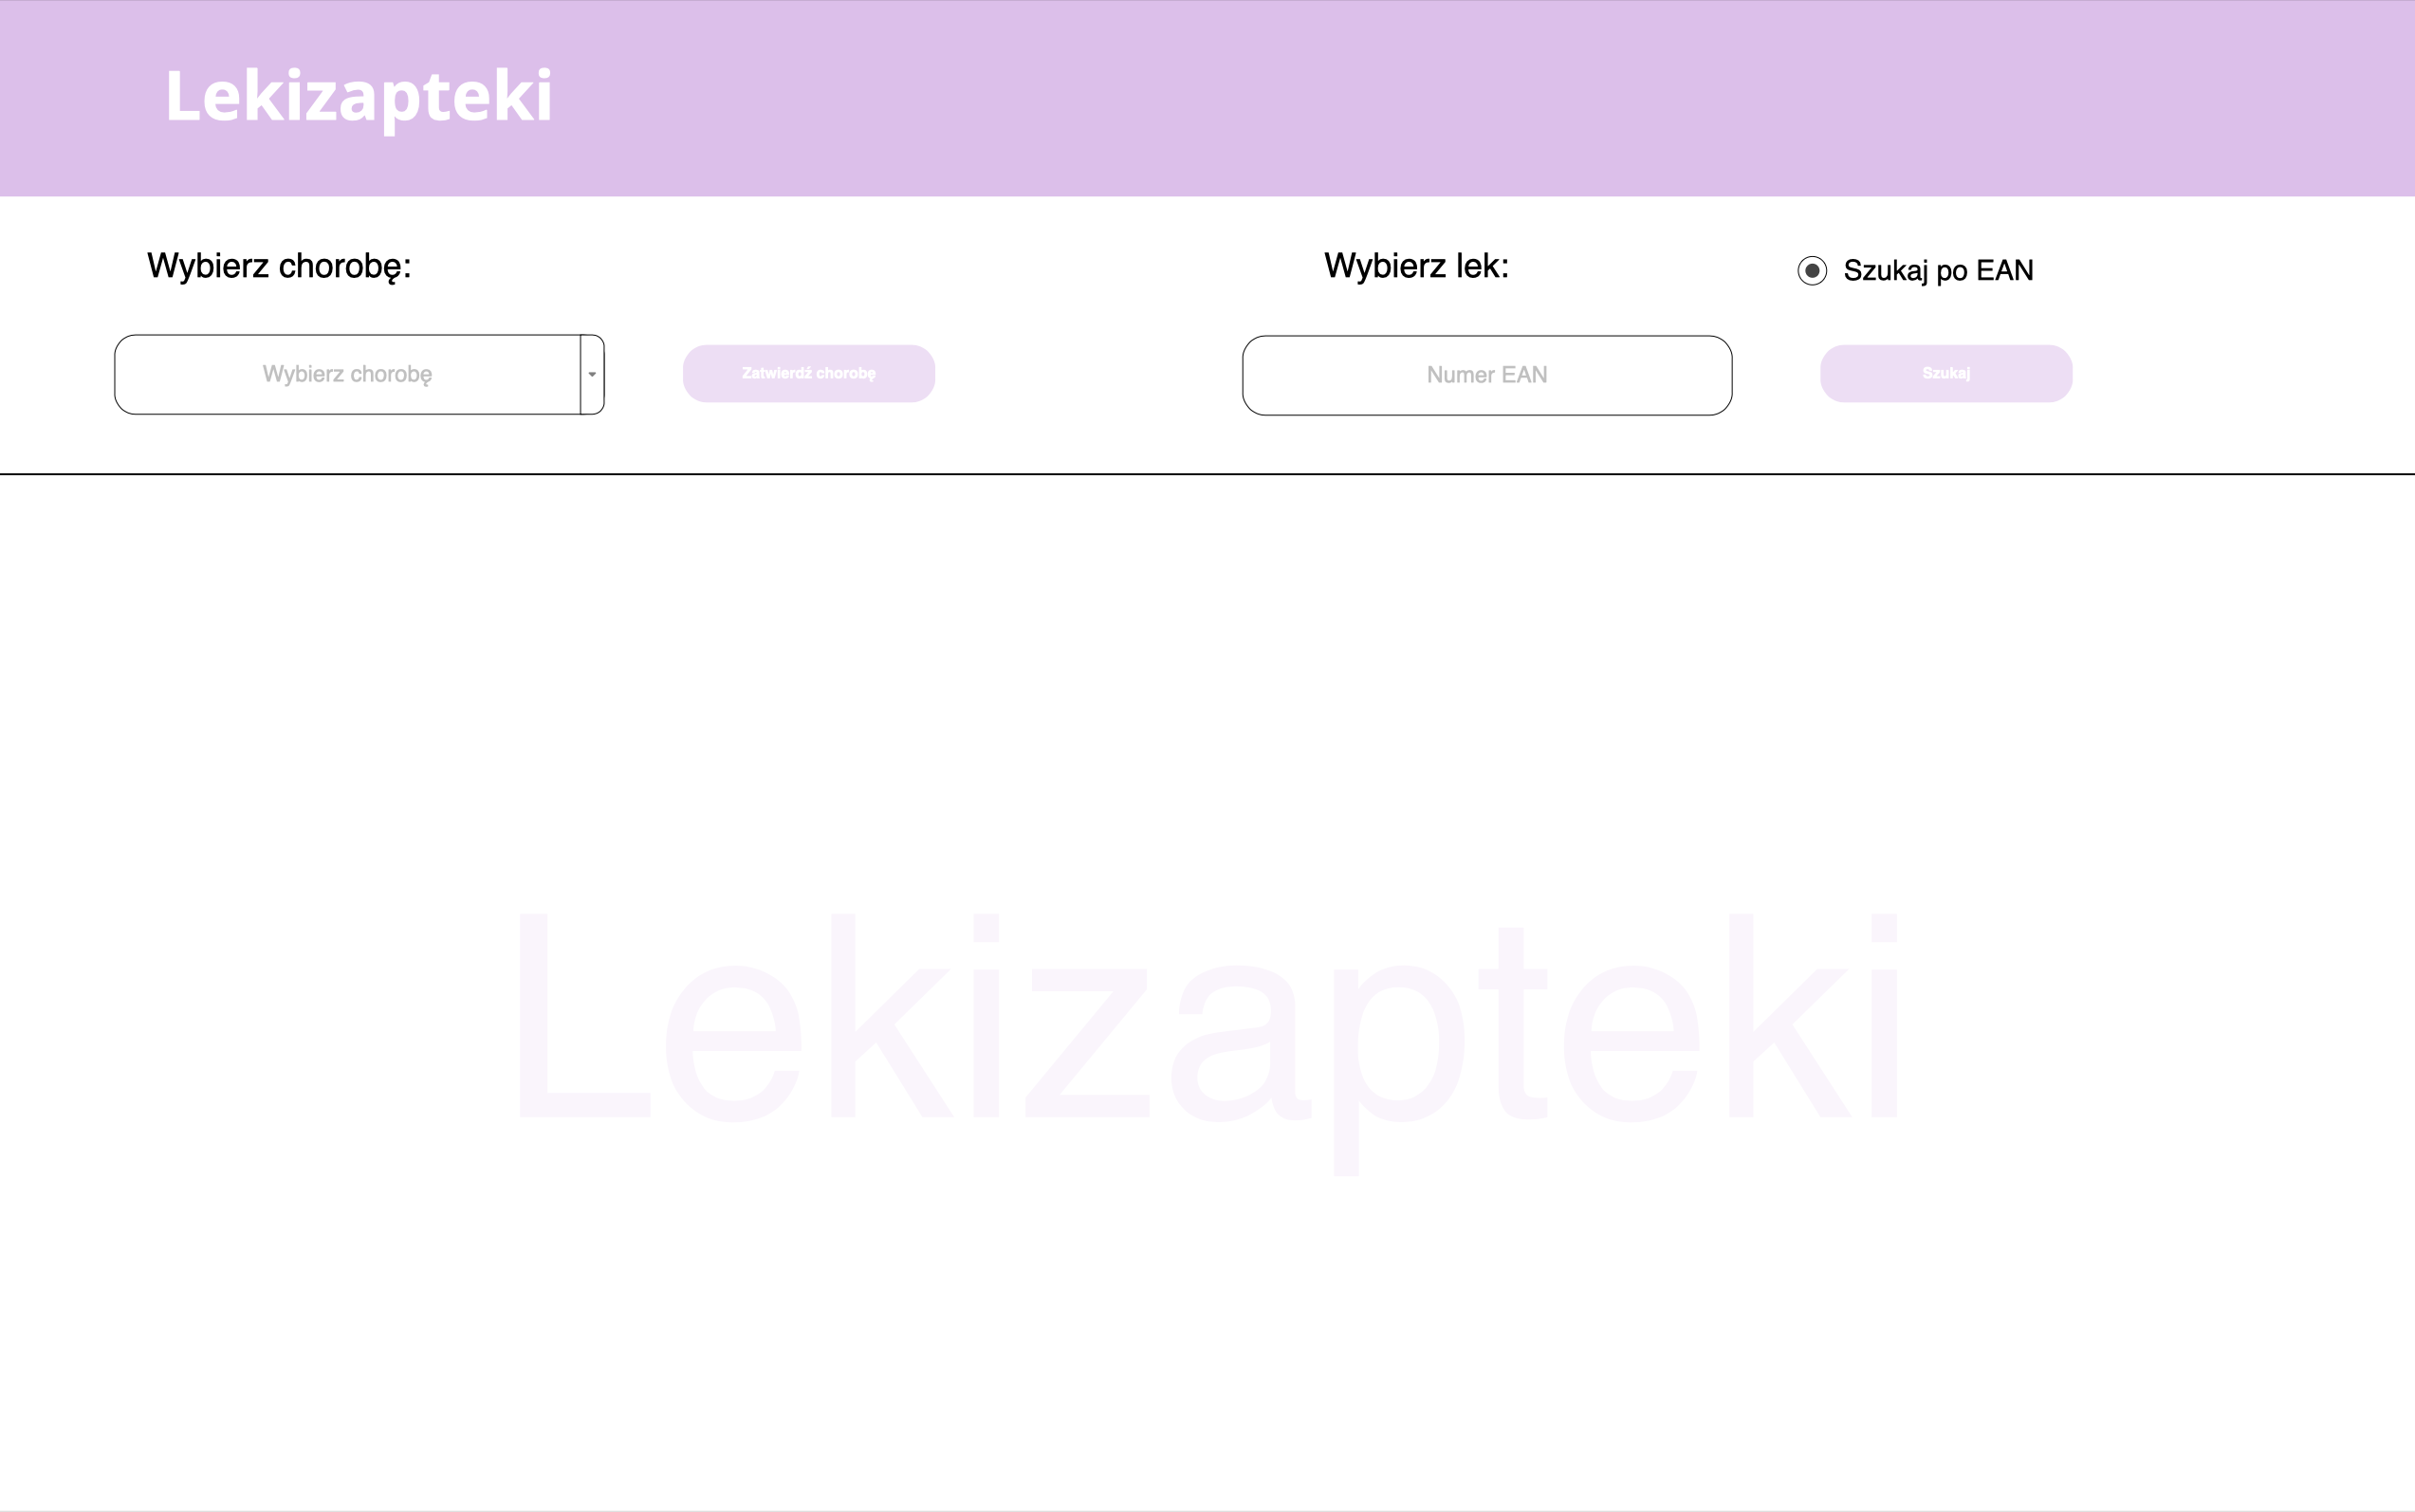
\includegraphics[width=8cm]{images/lekizapteki-wybor-leku-ean}

      \subsubsection{Wyniki i rozwinięte szczegóły dla pozycji}
      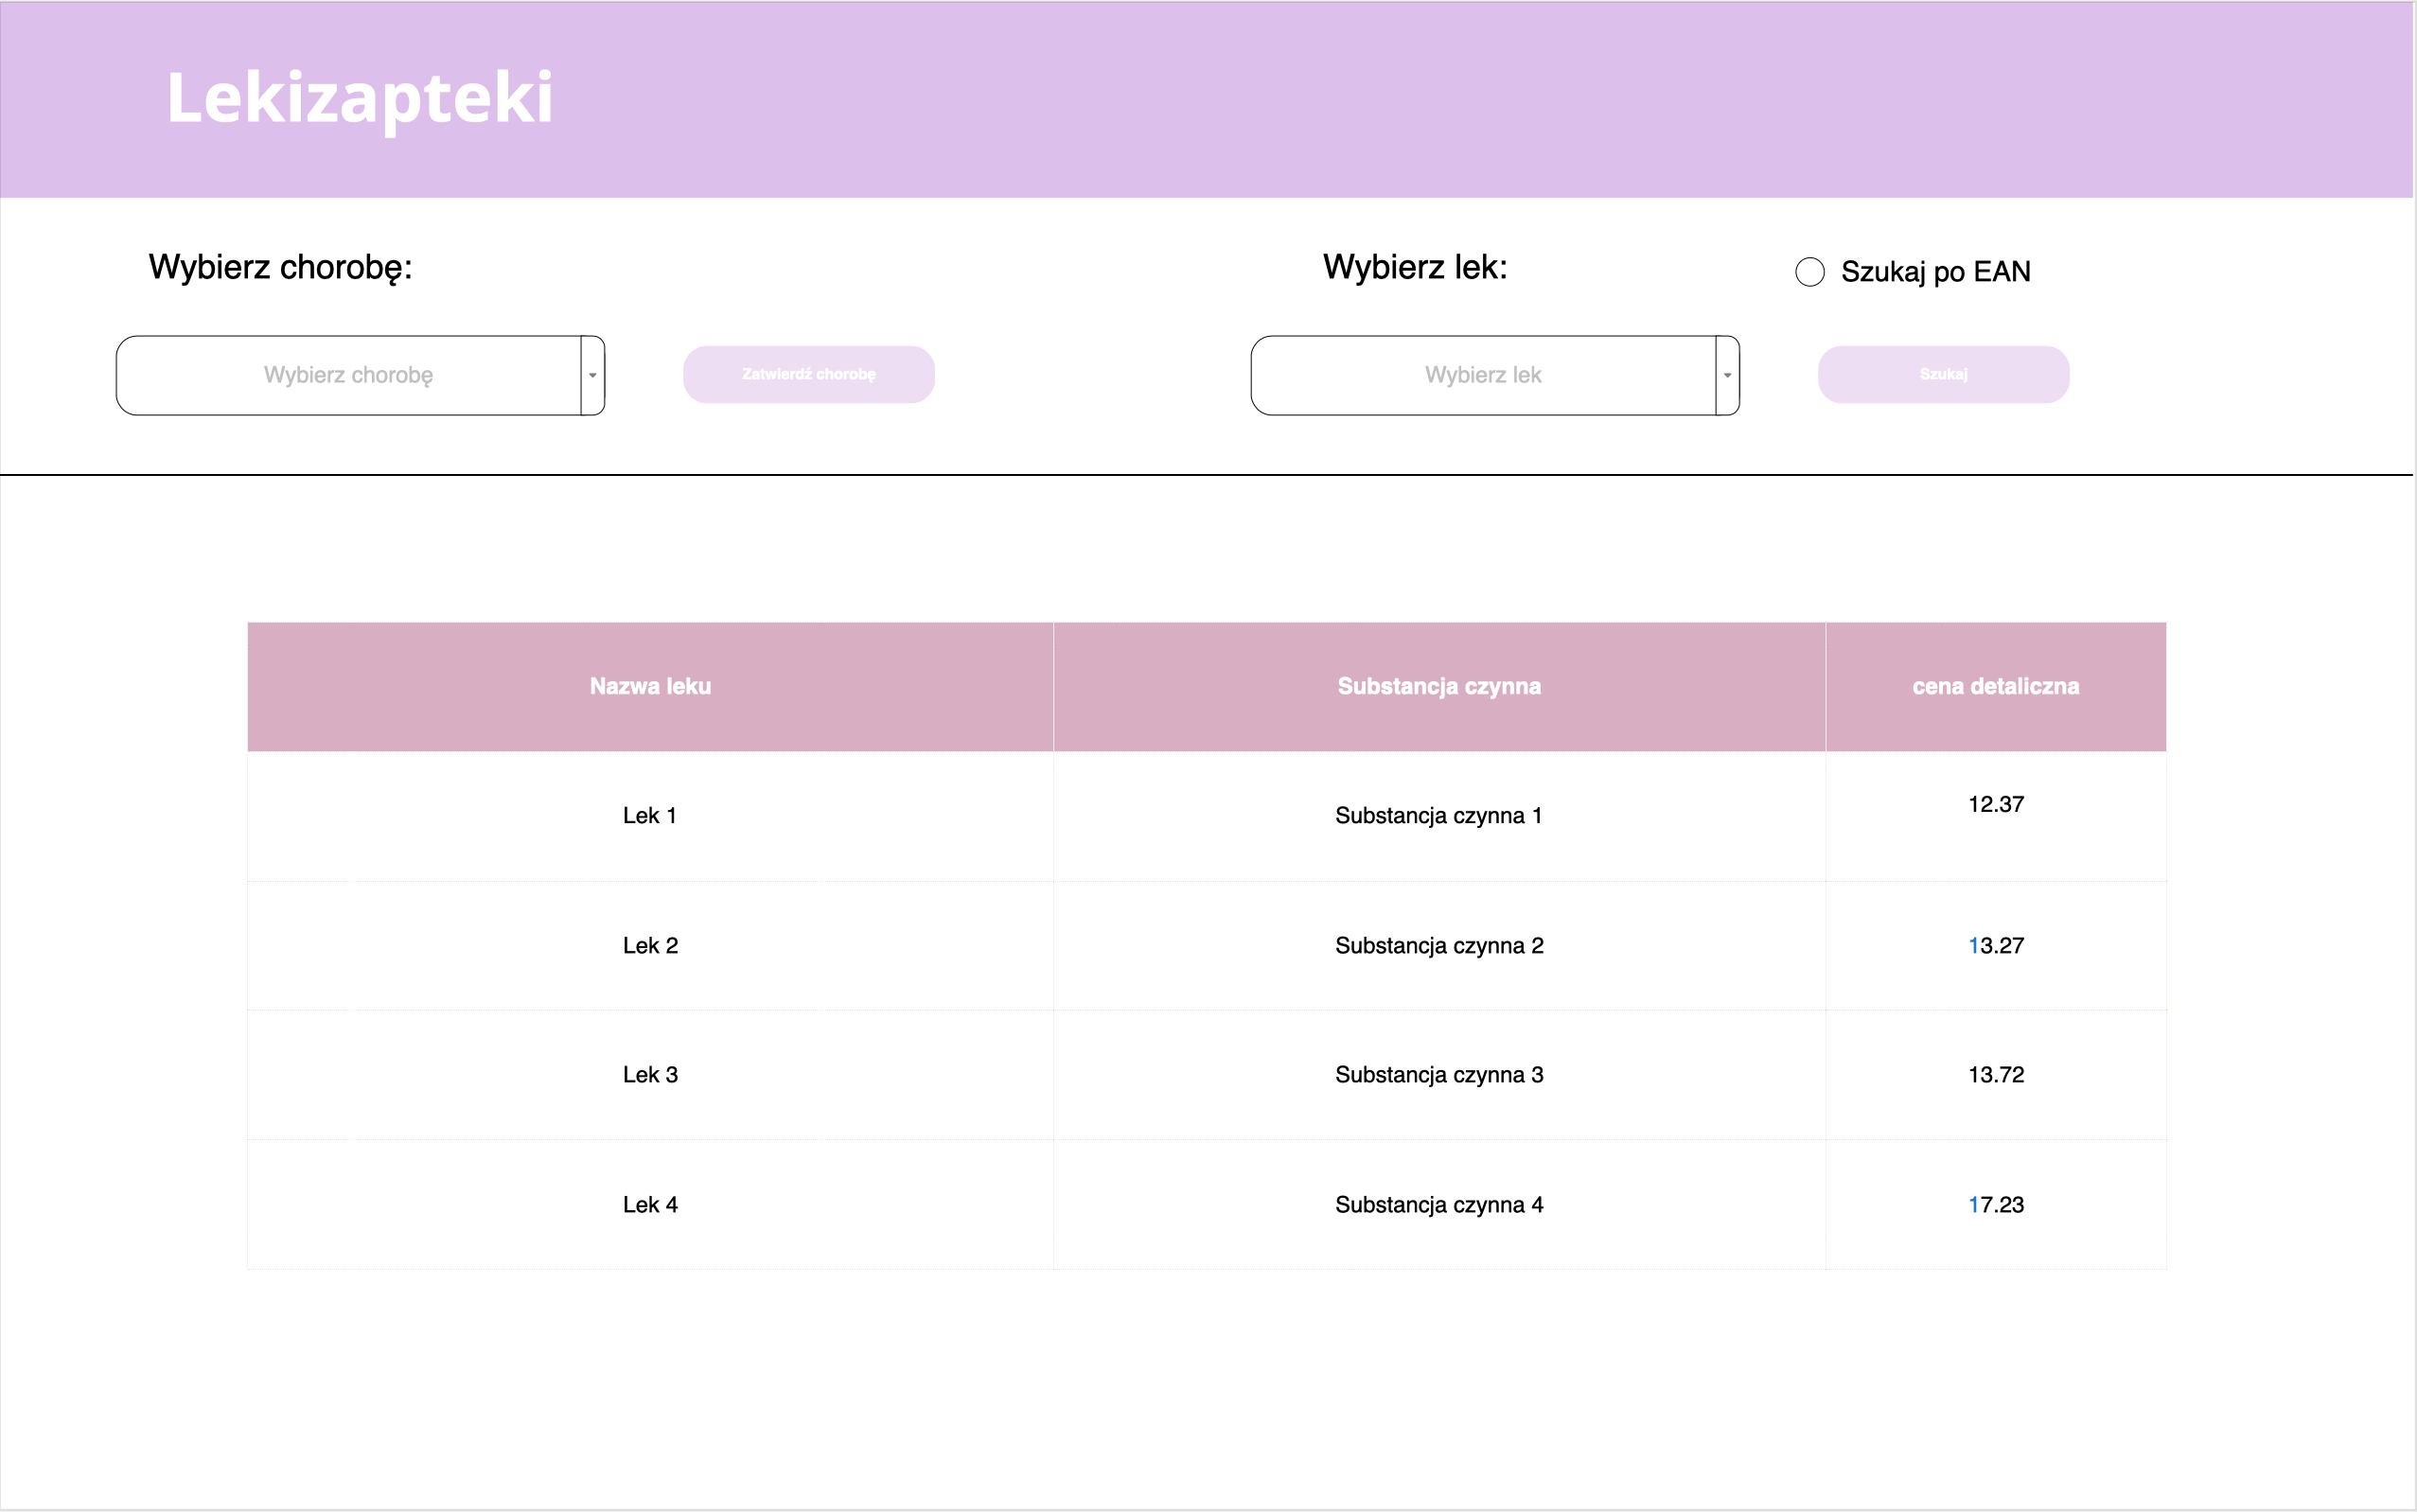
\includegraphics[width=8cm]{images/lekizapteki-leki-identyczne}
      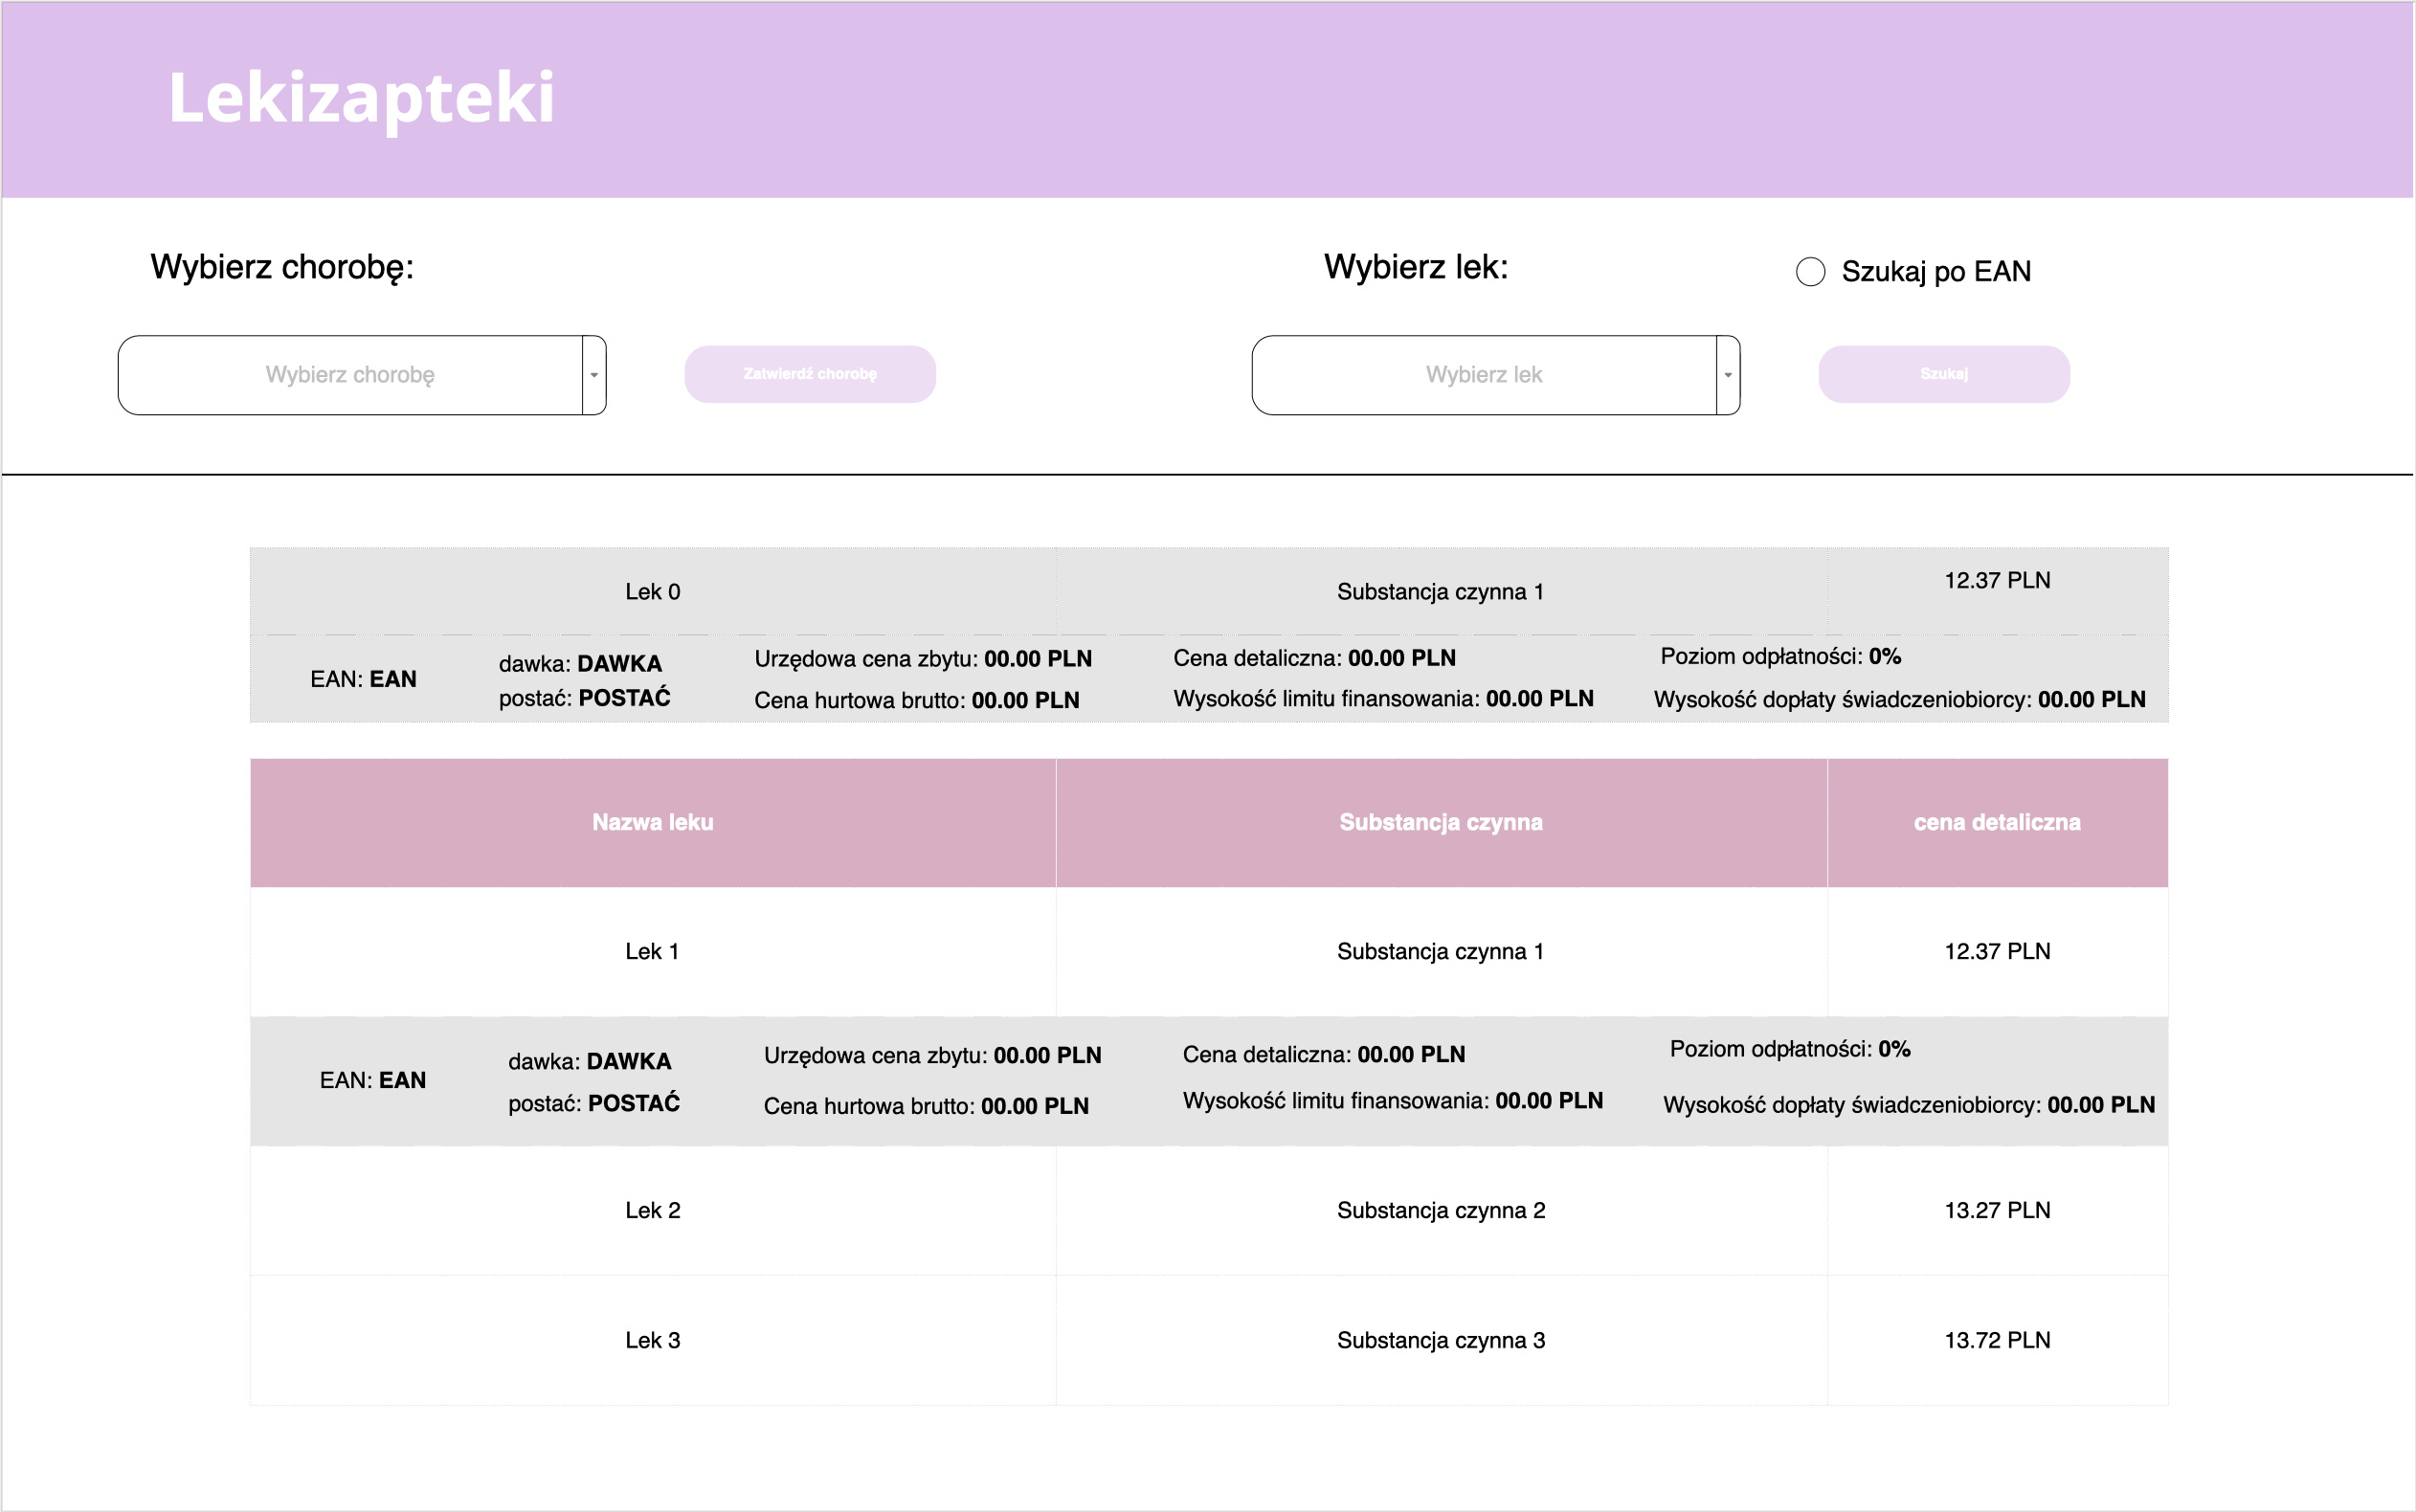
\includegraphics[width=8cm]{images/lekizapteki-leki-identyczne-rozwiniete}

  \section{Backend}
  Backend jest podzielony na dwa moduły: ``API'' i ``APP''.

    \subsection{Moduł API}
    Zawiera wystawione endpoint'y odpowiadające tym przedstawionym w punkcie 2.1.1.
    Są one w postaci interface'ów, klas z modelami oraz wyjątków rzucanych przy nieodpowiednich danych.

    \subsection{Moduł APP}
    Zawiera implementacje interface'ów z modułu API.
    Każdy interface jest implementowany przez kontroler.
    Kontrolery mają wstrzyknięte jedynie klasy służące do wykonywania pojedynczego endpointa (Command Pattern).

    Encje i relacje bazy danych są odwzorowane klasami z odpowiednimi adnotacjami.
    Zapytania do bazy danych odbywają się przez interface, implementowany przez framework,
    w którym nazwy metod są mapowane na zapytania do bazy danych.

    Dane z rozporządzeń są pobierane bezpośrednio przez aplikację w serwisie, który jest uruchamiany zaraz po powstaniu kontekstu.
    Może on pracować w dwóch trybach, które są konfigurowane w pliku \texttt{application.properties}.
    Pierwszym trybem jest pobieranie plików z podanego w konfiguracji linku,
    drugim jest pobieranie z lokalnego źródła, do którego ścieżka jest podana w konfiguracji.
    Parsuje on pliki z arkuszami Excel, waliduje, filtruje spełniające założenia serwisu oraz mapuje na encje w bazie danych.
  \section{Baza Danych}
  Baza danych jest \texttt{in-memory}, czyli jest tworzona przy tworzeniu kontekstu aplikacji.

  \subsection{Schemat}
    \noindent
    \begin{minipage}{.45\textwidth}
      \begin{lstlisting}
        CREATE TABLE DISEASE (
          id IDENTITY NOT NULL,
          name TEXT NOT NULL,

          CONSTRAINT disease_pk PRIMARY KEY (id)
        );

        CREATE TABLE INGREDIENT (
          id IDENTITY NOT NULL,
          name TEXT NOT NULL,

          CONSTRAINT ingredient_pky PRIMARY KEY (id)
        );

        CREATE TABLE DOSE (
          id IDENTITY NOT NULL,
          dose TEXT NOT NULL,

          CONSTRAINT dose_pk PRIMARY KEY (id)
        );

        CREATE TABLE FORM (
          id IDENTITY NOT NULL,
          name TEXT NOT NULL,

          CONSTRAINT form_pk PRIMARY KEY (id)
        );

        CREATE TABLE PACKAGE (
          id IDENTITY NOT NULL,
          content TEXT NOT NULL,

          CONSTRAINT package_pk PRIMARY KEY (id)
        );
      \end{lstlisting}
    \end{minipage}\hfill
    \begin{minipage}{.45\textwidth}
      \begin{lstlisting}
        CREATE TABLE PRICING (
          id IDENTITY NOT NULL,
          sale_price DECIMAL NOT NULL,
          retail_price DECIMAL NOT NULL,
          total_funding DECIMAL NOT NULL,
          charge_factor DECIMAL NOT NULL,
          refund DECIMAL NOT NULL,

          CONSTRAINT pricing_pk PRIMARY KEY (id)
        );

        CREATE TABLE MEDICINE (
          id IDENTITY NOT NULL,
          ean TEXT NOT NULL,
          name TEXT NOT NULL,
          dose_id NUMERIC NOT NUL,
          form_id NUMERIC NOT NUL,
          pricing_id NUMERIC NOT NUL,
          package_id NUMERIC NOT NUL,
          ingredient_id NUMERIC NOT NUL,
          disease_id NUMERIC NOT NUL,

          FOREIGN KEY (dose_id) REFERENCES DOSE (id),
          FOREIGN KEY (form_id) REFERENCES FORM (id),
          FOREIGN KEY (pricing_id) REFERENCES PRICING (id),
          FOREIGN KEY (package_id) REFERENCES PACKAGE (id),
          FOREIGN KEY (ingredient_id) REFERENCES INGREDIENT (id),
          FOREIGN KEY (disease_id) REFERENCES DISEASE (id),

          CONSTRAINT medicine_pk PRIMARY KEY (id)
        );
      \end{lstlisting}
    \end{minipage}

\end{document}
